%# -*- coding: utf-8-unix -*-
%%==================================================
%% chapter01.tex for SJTU Master Thesis
%%==================================================

%\bibliographystyle{sjtu2}%[此处用于每章都生产参考文献]
\chapter{提取地理位置特征}
\label{chap:Featu}



\section{选择地理位置特征}

O2O平台的用户发布评论的过程可以视为一个随机过程,发布评论的事件是以一个固定的概率稳定并独立发生的。在这个随机过程的。在这个过程下,评论相关的特征会遵循一些特殊的分布。例如著名的泊松过程下,时间间隔变量遵循泊松分布。在寻找帮助解决问题的特征时,研究目标特征遵循的分布特点十分有帮助。关于特征的选择,虽然已经有很多特征证明了它们在水军检测中的重要价值,例如时间、活跃量等,但是地理位置特征却被忽略了。分别计算普通用户和水军用户的地理位置特征的相关统计数据和分布特点,加以分析并寻找它们之间的不同之处,那么地理位置特征就可以成为解决问题的切入点。经过我们的研究调查,我们发现了一个可用的地理位置特征——“半径”:

\begin{defn}
	\textbf{半径}:每一个评论中店铺位置点和中心点的距离。其中中心点是一个用户的评论列表中最活跃地区内各个店铺位置的地理中心。中心点被视为该用户的居所。
\end{defn}

图~\ref{fig:radius}是半径特征的示例,图中标有REVIEW LOCATION的点是一个用户写过评论的各个店铺的位置,标有CENTER的点便是这些店铺位置的地理中心。我们认为这个点便是该用户平时居住的地方。图中连接CENTER点和各个REVIEW LOCATION点的线代表了这些点的间隔距离,也就是每个店铺对应半径特征的值。

\begin{figure}[htbp]
	\centering
	\begin{minipage}[htbp]{0.6\textwidth}
		\centering
		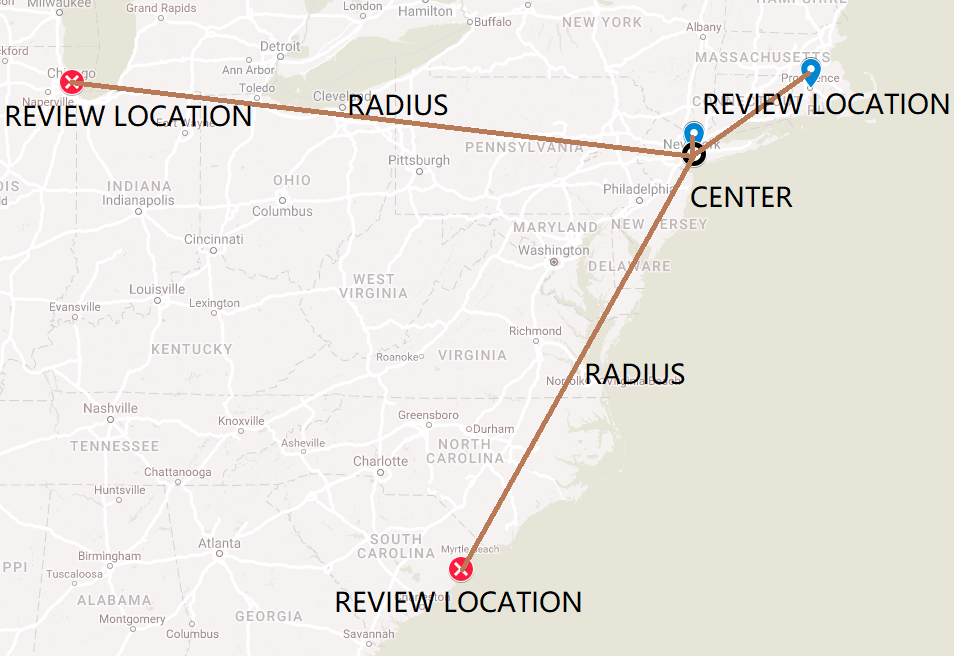
\includegraphics[width=10cm]{featu-1.png}
		\caption[地理位置特征“半径”示意图]
		{地理位置特征“半径”示意图(图源:谷歌地图)\label{fig:radius}}		
	\end{minipage}     
\end{figure}



\section{半径特征的合理性论述}

表~\ref{tbl:radius}和图~\ref{fig:hist}展示了半径特征的统计数据和频率分布直方图。计算数据来源于我们使用的数据集。统计数据中的平均值和标准差表现了半径特征在两类用户之间的差异。频率分布直方图更加具体地展示了水军用户(Spammer)和普通用户(Non-spammer)的差异,包括图像各位置的斜率、各顶点位置等。但是二者的图像也有相似的部分,那就是它们都呈现出了双峰分布的趋势。而这种双峰图像的形成过程可以看做是两个参数不同的高斯分布(Gaussian Distribution)在对数横坐标轴上的叠加。

\begin{table}[htbp]
	\caption{半径特征的统计数据}
	\label{tbl:radius}
	\centering
	\begin{tabular}{ccc}
		\toprule
		& 平均值 & 标准差  \\
		\midrule
		水军用户      & 310.0604  & 678.4959  \\
		普通用户  & 568.5133  &	999.4281 \\
		\bottomrule
	\end{tabular}
\end{table}

\begin{figure}[htbp]
	\centering
	\begin{minipage}[htbp]{0.6\textwidth}
		\centering
		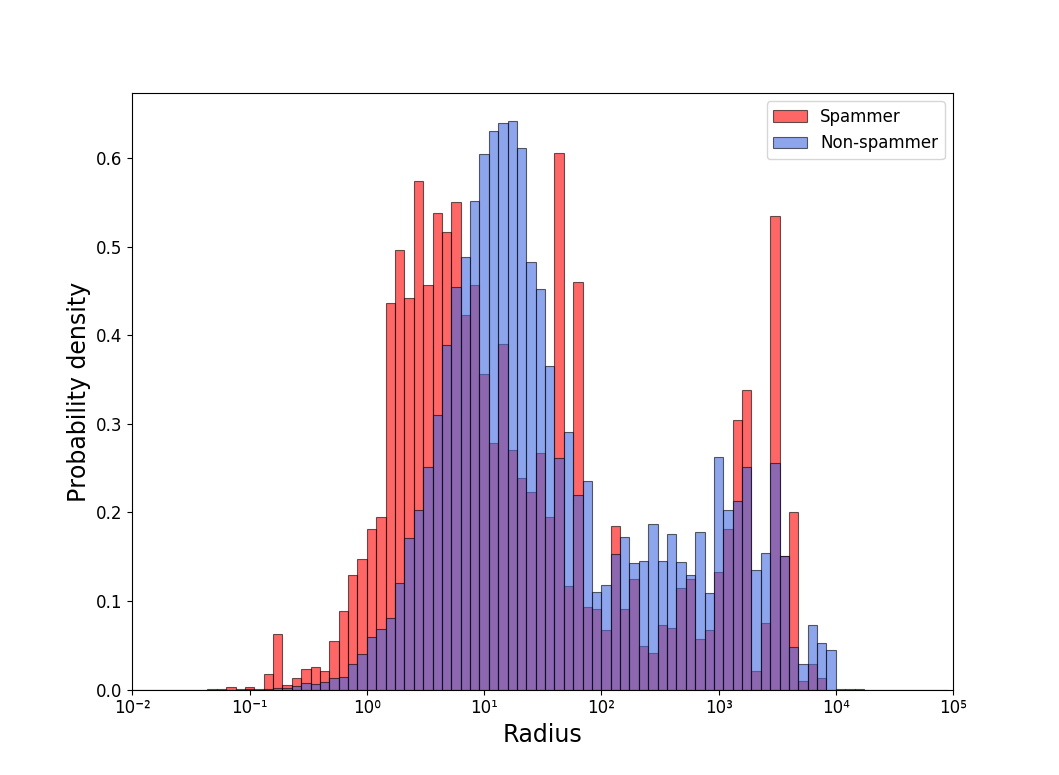
\includegraphics[width=10cm]{featu-2.png}
		\caption[半径特征的频率分布图]
		{半径特征的频率分布图\label{fig:hist}}		
	\end{minipage}     
\end{figure}

从水军用户和普通用户的行为上分析,这种双峰分布是合理的。总体来看,人类的活动范围可以分为两个模式:近距离活动和远距离活动。近距离活动就是人类在居所的附近活动,这类活动占比最高,活动范围不会很远,通常在一个城市的范围之内;远距离活动一般出现在一个人离开居所很长时间的时候,例如旅游、出差等,这类活动的地理位置跨越范围较大,但持续时间不会太长。故普通用户图像中的双峰是近距离活动和远距离活动的合理体现。然而,水军用户并不符合近距离活动和远距离活动的模式,他们的行动模式是无规律的,水军用户的双峰图像只是其进行水军活动时不同半径的店铺数量占比的体现。此外,普通用户和水军用户在评论店铺的半径特征顺序上也是有差异的。普通用户评论过的店铺中,连续的店铺的半径特征值基本上是相近的。换句话说,普通用户在店铺的选择上具有空间连续性。这是因为人类的行动是具有空间连续性的,人们在一段时间内是在同一片区域生活的,所以人类日常消费的场所是接近的。即使短时间内出远门旅行,在旅行中的消费场所也是接近的。反观水军用户,其评论店铺的顺序是由雇主要求决定的而非人类正常活动,所以他们的半径特征不具有空间连续性。这两点关键差异将是SpamTracer模型进行水军检测的重要依据。

接下来对半径特征进行数学角度的建模。如上文所提到的,我们用两个参数不同的高斯分布的叠加来描述半径特征的频率分布。假设$x_i, i = 1,...,T$是一个用户的评论列表中按时间排序出现的店铺位置,根据公式~\eqref{equation:1},我们计算其地理中心$C$,然后计算每一个评论的店铺所对应的半径特征值$\gamma_{x_i}$。半径特征值$\gamma_{x_i}$遵循高斯分布。


\begin{equation}
\label{equation:1}
\begin{aligned}
& C = (\frac{\sum_{t \in T}{x_t.latitude}}{|T|}, \frac{\sum_{t \in T}{x_t.longitude}}{|T|})\\
& \gamma_{x_i} = Distance(x_i, C)\\
& f(x;\mu, \sigma) = \frac{1}{\sqrt{2\pi}\sigma}\exp{(-\frac{(x-\mu)^2}{2\sigma^2})} \qquad
\gamma_{x}\sim N(\mu, \sigma^2) \\
\end{aligned}
\end{equation}